%%%%%%%%%%%%%%%%%%%%%%%%%%%%%%%%%%%%%%%%%%%%%%%%%%%%%%%%%%%%%%%%%%%%%%%%%
% This file is part of the LaTeX sources of the OMDoc 1.3 specification
% Copyright (c) 2016 Michael Kohlhase.
% Source at https://github.com/KWARC/OMDoc/tree/master/doc/spec
% This work is licensed by the Creative Commons Share-Alike license
% see http://creativecommons.org/licenses/by-sa/2.5/ for details
%%%%%%%%%%%%%%%%%%%%%%%%%%%%%%%%%%%%%%%%%%%%%%%%%%%%%%%%%%%%%%%%%%%%%%%%%

\begin{tchapter}[id=natlist]{Structured and Parametrized Theories}
  
In {\mychapref{omcds}} we have seen a simple use of theories in {\openmath} content
dictionaries. There, theories have been used to reference {\openmath} symbols and to
govern their visibility. In this chapter we will cover an extended example showing the
structured definition of multiple mathematical theories, modularizing and re-using parts
of {\indextoo{specification}s} and theories\index{theory}.  Concretely, we will consider a
structured specification of lists of natural numbers. This example has been used as a
paradigmatic example for many specification formats ranging from {\casl} (Common Abstract
Specification Language~\cite{CoFI:2004:CASL-RM}) standard to the {\pvs} theorem prover~\cite{OwRu92},
since it uses most language elements without becoming too unwieldy to present.

\begin{myfig}{natlist:actualization}{A Structured Specification of Lists (of
    Natural Numbers)}
  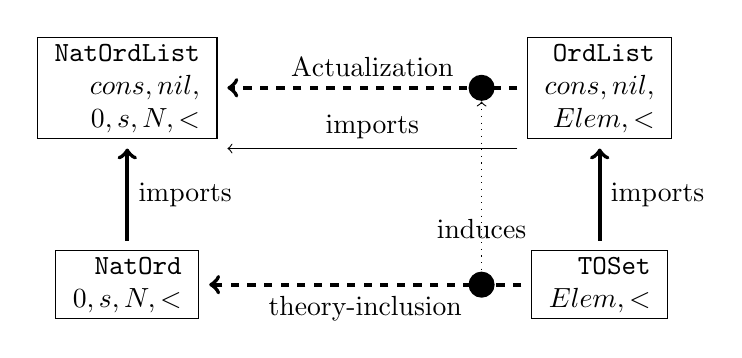
\begin{tikzpicture}  \node (natordlist) at (0,2.5) 
    {\begin{tabular}{|r|}\hline 
      {\tt{NatOrdList}}\\
      $cons, nil,$\\
      $0,s,{\mathbb{N}},<$\\\hline
    \end{tabular}};
  \node (natord) at (0,0) 
    {\begin{tabular}{|r|}\hline 
      {\tt{NatOrd}}\\
      $0,s,{\mathbb{N}},<$\\\hline
    \end{tabular}};
  \node (toset) at (6,0) 
    {\begin{tabular}{|r|}\hline 
      {\tt{TOSet}}\\
      $Elem,<$\\\hline
    \end{tabular}};
  \node (ordlist) at (6,2.5) 
    {\begin{tabular}{|r|}\hline 
      {\tt{OrdList}}\\
      $cons, nil,$\\
      $Elem,<$\\\hline
    \end{tabular}};
  \node[circle,fill] (act1) at (4.5,2.5) {};
  \node[circle,fill] (act2) at (4.5,0) {};
  \draw [->,line width=1.5pt] (natord) -- node[right]{imports} (natordlist);
  \draw [->,line width=1.5pt] (toset) -- node[right]{imports} (ordlist);
  \draw [->,dashed,line width=1.5pt] (toset) -- node[below]{theory-inclusion} (natord);
  \draw [->,dashed,line width=1.5pt] (ordlist) -- node[above]{Actualization} (natordlist);
  \draw [->] (ordlist.south west) -- node[above]{imports} (natordlist.south east);
  \draw [<-,dotted,near end] (act1) -- node{induces} (act2);
\end{tikzpicture}
\end{myfig}

In this example, we specify a theory {\snippet{OrdList}} of lists that is generic in the
elements (which is assumed to be a totally ordered set, since we want to talk about
ordered lists).  Then we will instantiate {\snippet{OrdList}} by applying it to the theory
{\snippet{NatOrd}} of natural numbers to obtain the intended theory {\snippet{NatOrdList}} of
lists of natural numbers.  The advantage of this approach is that we can re-use the
generic theory {\snippet{OrdList}} to apply it to other element theories like that of
``characters'' to obtain a theory of lists of characters.  In
{\twintoo{algebraic}{specification}} languages, we speak of {\defemph{parametric
    theories}}\twin{parametric}{theory}.  Here, the theory {\snippet{OrdList}} has a formal
{\indextoo{parameter}} (the theory {\snippet{TOSet}}) that can be instantiated later with
concrete values to get a {\twindef{theory}{instance}} (in our example the theory
{\snippet{NatOrdList}}).  We call this process theory {\defin{actualization}}.

We begin the extended example with the theories in the lower half of
{\myfigref{natlist:actualization}}.  The first is a (mock up of a) theory of totally
ordered sets. Then we build up the theory of natural numbers as an
{\twindef{abstract}{data type}} (see {\mychapref{adt}} for an introduction to abstract
data types in {\omdoc} and a more elaborate definition of $\mathbb N$). The
{\element{sortdef}} element posits that the set of natural numbers is given as the
{\defin{sort}} {\snippet{NatOrd}}, with the {\indextoo{constructor}s} {\snippet{zero}} and
{\snippet{succ}}. Intuitively, a sort represents an {\twintoo{inductively defined}{set}},
i.e. it contains exactly those objects that can be represented by the constructors only,
for instance the number three is represented as $s(s(s(0)))$, where $s$ stands for the
successor function (given as the constructor {\snippet{succ}}) and $0$ for the number zero
(represented by the constructor {\snippet{zero}}). Note that the theory {\snippet{nat}}
does not have any explicitly represented axioms. They are implicitly given by the abstract
data type structure, in our case, they correspond to the five Peano Axioms (see
{\myfigref{peano}}).  Finally, the {\element{argument}} elements also introduce one
partial inverse to the constructor functions per argument; in our case the
{\twintoo{predecessor}{function}}.

\begin{lstlisting}[mathescape,label=lst:nat-param,
  index={theory,symbol,definition,assertion}]
<theory xml:id="TOSet">                   
  <symbol name="set"/>
  <symbol name="ord"/>
  <axiom xml:id="toset"><CMP><xhtml:p>$ord$ is a  total order on $set$.</xhtml:p></CMP></axiom>
</theory>                               

<theory xml:id="nat">
  <adt>
    <sortdef name="Nat">
      <constructor name="zero"/>
      <constructor name="succ">
        <argument>
          <type><OMOBJ><OMS name="Nat" cd="nat"/></OMOBJ></type>
          <selector name="pred"/>
        </argument>
      </constructor>
    </sortdef>
  </adt>
</theory>

<theory xml:id="NatOrd">
  <imports from="#nat"/>
  <imports from="#TOSet"/>
  <symbol name="leq"/>
  <definition xml:id="leq.def" for="leq" type="implicit" 
              existence="#leq.ex" uniqueness="#leq.uniq">
    <FMP>$\allcdot{x}{0\leq x}\land\allcdot{x,y}{x\leq y\implies s(x)\leq s(y)}$</FMP>
  </definition>
  <assertion xml:id="leq.ex"><CMP><xhtml:p>$\leq$ exists.</xhtml:p></CMP></assertion>
  <assertion xml:id="leq.unique"><CMP><xhtml:p>$\leq$ is unique.</xhtml:p></CMP></assertion>
  <assertion xml:id="leq.TO"><CMP><xhtml:p>$\leq$ is a  total order on $Nat$.<xhtml:p></CMP></assertion>
</theory>                       
\end{lstlisting}

Finally we have extended the natural numbers by an ordering function $\leq$ (symbol
{\snippet{leq}}) which we show to be a total ordering function in assertion
{\snippet{leq.TO}}.  Note that to state the assertion, we had to import the notion of a
total ordering from theory {\snippet{TOSet}}. We can directly use this result to establish
a {\twindef{theory}{inclusion}} between {\snippet{TOSet}} as the
{\twindef{source}{theory}} and {\snippet{NatOrd}} as the {\twindef{target}{theory}}. A
{\twintoo{theory}{inclusion}} is a formula mapping between two theories, such that the
translations of all axioms in the {\twintoo{source}{theory}} are provable in the
{\twintoo{target}{theory}}. In our case, the mapping is given by the recursive function
given in the {\element{morphism}} element in {\mylstref{nat-ti}} that maps the respective
base sets and the ordering relations to each other. The {\element{obligation}} element
just states that translation of the only theory-constitutive
(see \mysubsecref{definitions}) element of the source theory (the axiom
{\snippet{toset}}) has been proven in the target theory, as witnessed
by the assertion {\snippet{leq.TO}}\footnote{Note that as always,
  {\omdoc} only cares about the structural aspects of this: The
  {\omdoc} model only insists that there is the statement of an
  assertion, whether the author chooses to prove it or indeed whether
  the statement is true at all is left to other levels of modeling.}.

\begin{lstlisting}[mathescape,label=lst:nat-ti,
  index={theory,symbol,definition,assertion}]
<theory-inclusion xml:id="elem-nat-incl" to="#NatOrd" from="#TOSet">
  <morphism xml:id="elem-nat" type="pattern">
    <requation>
      <OMOBJ><OMS cd="TOSet" name="set"/></OMOBJ>
      <OMOBJ><OMS cd="NatOrd" name="Nat"/></OMOBJ>
    </requation>
    <requation>
      <OMOBJ><OMS cd="TOSet" name="ord"/></OMOBJ>
      <OMOBJ><OMS cd="NatOrd" name="leq"/></OMOBJ>
    </requation>
  </morphism>
  <obligation induced-by="#toset" assertion="#leq.TO"/>
</theory-inclusion>
\end{lstlisting}

We continue our example by building a generic theory {\snippet{OrdList}} of ordered lists.
This is given as the abstract data type generated by the symbols {\snippet{cons}}
(construct a list from an element and a rest list) and {\snippet{nil}} (the empty list)
together with a defined symbol {\snippet{ordered}}: a predicate for ordered lists. Note
that this symbol cannot be given in the abstract data type, since it is not a constructor
symbol. Note that {\snippet{OrdList}} imports theory {\snippet{TOSet}} for the base set of
the lists and the ordering relation $\leq$.

\begin{lstlisting}[mathescape,label=ordered-list,
  index={theory,imports,adt,sortdef,constructor,argument,symbol,definition}]
<theory xml:id="OrdList">
  <imports from="#TOSet"/>
  <adt xml:id="list-adt">
    <sortdef name="lists">
      <constructor name="cons">
        <argument>
          <type><OMOBJ><OMS name="set" cd="TOSet"/></OMOBJ></type>
          <selector name="head"/>
        </argument>
        <argument>
          <type><OMOBJ><OMS name="lists" cd="OrdList"/></OMOBJ></type>
          <selector name="rest"/>
        </argument>
      </constructor>
      <constructor name="nil"/>
    </sortdef>
  </adt>

  <symbol name="ordered"/>
  <definition xml:id="ordered-def" for="ordered" type="informal">
    <CMP><xhtml:p>A list $l$ is called ordered, iff $head(l)\leq z$ for all elements $z\in rest(l)$ and
    $rest(l)$ is ordered.</xhtml:p></CMP>
  </definition>
</theory>
\end{lstlisting}

The theory {\snippet{NatOrdList}} of lists of natural numbers is built up by
importing from the theories {\snippet{NatOrd}} and {\snippet{OrdList}}. Note that the
attribute {\attribute{type}{imports}} of the {\element{imports}} element
{\snippet{nat-list.im-elt}} is set to {\attval{local}{type}{imports}}, since we
only want to import the local axioms of the theory {\snippet{OrdList}} and not the
whole theory {\snippet{OrdList}} (which would include the axioms from
{\snippet{TOSet}}; see {\mysecref{restricting-inference}} for a discussion). In
particular the symbols {\snippet{set}} and {\snippet{ord}} are not imported into
theory {\snippet{NatOrdList}}: the theory {\snippet{TOSet}} is considered as a
{\atwindef{formal}{parameter}{theory}}, which is actualized to the
{\atwindef{actual}{parameter}{theory}} with this construction.  The effect of the
actualization comes from the morphism {\snippet{elem-nat}} in the import of
{\snippet{OrdList}} that renames the symbol {\snippet{set}} (from theory
{\snippet{TOSet}}) with {\snippet{Nat}} (from theory {\snippet{NatOrd}}). The
actualization from {\snippet{OrdList}} to {\snippet{NatOrdList}} only makes sense, if
the parameter theory {\snippet{NatOrd}} also has a suitable ordering function.  This
can be ensured using the {\omdoc} {\element{inclusion}} element.

\begin{lstlisting}[mathescape,label=lst:nat-list,
  index={theory,imports,morphism,inclusion}]
<theory xml:id="NatOrdList">
  <imports xml:id="natordlist.im-natord" from="#NatOrd"/>
  <imports xml:id="natordlist.im-elt" from="#OrdList" type="local">
    <morphism base="#elem-nat"/>
  </imports>
  <inclusion via="elem-nat-incl"/>
</theory>
\end{lstlisting}
The benefit of this {\element{inclusion}} requirement is twofold: If the theory inclusion
from {\snippet{TOSet}} to {\snippet{NatOrd}} cannot be verified, then the theory
{\snippet{NatOrdList}} is considered to be undefined, and we can use the
{\twintoo{development}{graph}} techniques presented in {\mysecref{development-graphs}} to
obtain a theory inclusion from {\snippet{OrdList}} to {\snippet{NatOrdList}}: We first
establish an axiom inclusion from theory {\snippet{TOSet}} to {\snippet{NatOrdList}} by
observing that this is induced by composing the theory inclusion from {\snippet{TOSet}} to
{\snippet{NatOrd}} with the theory inclusion given by the {\element{imports}} from
{\snippet{NatOrd}} to {\snippet{NatOrdList}}. This gives us a
{\defin{decomposition}} situation: every theory that the source theory {\snippet{OrdList}}
inherits from has an axiom inclusion to the target theory {\snippet{NatOrdList}}, so the
local axioms of those theories are provable in the target theory. Since we have covered
all of the inherited ones, we actually have a theory inclusion from the source- to the
target theory.

\begin{lstlisting}[mathescape,label=lst:nat-list-inclusions,
  index={theory,imports,morphism,inclusion}]
<axiom-inclusion xml:id="toset-natordlist-incl" from="#TOSet" to="#NatOrdList">
  <morphism base="#elem-nat"/>
  <path-just local="#elem-nat-incl" globals="#natordlist.im-natord"/>
</axiom-inclusion>

<theory-inclusion from="#OrdList" to="#NatOrdList">
  <morphism base="#elem-nat"/>
  <decomposition links="#toset-natordlist-incl #elem-nat-incl"/>
</theory-inclusion>
\end{lstlisting}

This concludes our example, since we have seen that the theory {\snippet{OrdList}} is
indeed included in {\snippet{NatOrdList}} via renaming.

Note that with this construction we could simply extend the graph by actualizations for
other theories, e.g. to get {\twintoo{lists of}{character}s}, as long as we can prove
{\twintoo{theory}{inclusion}s} from {\snippet{TOSet}} to them.
\end{tchapter}

%%% Local Variables: 
%%% mode: latex
%%% TeX-master: "omdoc"
%%% End: 

% LocalWords:  natlist omcds TOSet adt sortdef succ nat peano mathescape lst ti
% LocalWords:  param ord toset pred NatOrd def uniq elem incl requation cd nats
% LocalWords:  OrdList im NatOrdList elt natordlist leq ns attr natord toset
% LocalWords:  toset CMP OMOBJ FMP toset natordlist natord natordlist toset

% LocalWords:  natordlist natord natordlist toset natordlist globals natordlist
% LocalWords:  natord toset natordlist toset toset toset natordlist natord
% LocalWords:  natordlist toset natordlist natordlist natord toset natordlist
% LocalWords:  toset toset toset natordlist natord natordlist toset natordlist
% LocalWords:  natordlist natord toset natordlist
